
\section{Insegnante}

\subsection{UC2.1 Registrazione insegnanti}

\begin{itemize}
	\item[•] \textbf{Attori}: 
	\item[•] \textbf{Descrizione}:
	\item[•] \textbf{Precondizione}:
	\item[•] \textbf{Postcondizione}:
	\item[•] \textbf{Flusso degli eventi}:
		\begin{enumerate}
			\item
			\item
		\end{enumerate}
	\item[•] \textbf{Estensioni}:
		\begin{enumerate}
			\item
			\item
		\end{enumerate}
\end{itemize}

\subsection{UC2.1.1 Inserimento nome utente}
\begin{itemize}
	\item[•] \textbf{Attori}: 
	\item[•] \textbf{Descrizione}:
	\item[•] \textbf{Precondizione}:
	\item[•] \textbf{Postcondizione}:
	\item[•] \textbf{Flusso degli eventi}:
		\begin{enumerate}
			\item
			\item
		\end{enumerate}
	\item[•] \textbf{Estensioni}:
		\begin{enumerate}
			\item
			\item
		\end{enumerate}
\end{itemize}

\subsection{UC2.1.2 Inserimento email istituzionale}
\begin{itemize}
	\item[•] \textbf{Attori}: 
	\item[•] \textbf{Descrizione}:
	\item[•] \textbf{Precondizione}:
	\item[•] \textbf{Postcondizione}:
	\item[•] \textbf{Flusso degli eventi}:
		\begin{enumerate}
			\item
			\item
		\end{enumerate}
	\item[•] \textbf{Estensioni}:
		\begin{enumerate}
			\item
			\item
		\end{enumerate}
\end{itemize}

\subsection{UC2.1.3 Inserimento password}
\begin{itemize}
	\item[•] \textbf{Attori}: 
	\item[•] \textbf{Descrizione}:
	\item[•] \textbf{Precondizione}:
	\item[•] \textbf{Postcondizione}:
	\item[•] \textbf{Flusso degli eventi}:
		\begin{enumerate}
			\item
			\item
		\end{enumerate}
	\item[•] \textbf{Estensioni}:
		\begin{enumerate}
			\item
			\item
		\end{enumerate}
\end{itemize}

\subsection{UC2.1.5 Inserimento data di nascita}
\begin{itemize}
	\item[•] \textbf{Attori}: 
	\item[•] \textbf{Descrizione}:
	\item[•] \textbf{Precondizione}:
	\item[•] \textbf{Postcondizione}:
	\item[•] \textbf{Flusso degli eventi}:
		\begin{enumerate}
			\item
			\item
		\end{enumerate}
	\item[•] \textbf{Estensioni}:
		\begin{enumerate}
			\item
			\item
		\end{enumerate}
\end{itemize}

\subsection{UC2.1.6 Inserimento scuola di appartenenza}
\begin{itemize}
	\item[•] \textbf{Attori}: 
	\item[•] \textbf{Descrizione}:
	\item[•] \textbf{Precondizione}:
	\item[•] \textbf{Postcondizione}:
	\item[•] \textbf{Flusso degli eventi}:
		\begin{enumerate}
			\item
			\item
		\end{enumerate}
	\item[•] \textbf{Estensioni}:
		\begin{enumerate}
			\item
			\item
		\end{enumerate}
\end{itemize}

\subsection{UC2.1.7 Inserimento materia insegnata}
\begin{itemize}
	\item[•] \textbf{Attori}: 
	\item[•] \textbf{Descrizione}:
	\item[•] \textbf{Precondizione}:
	\item[•] \textbf{Postcondizione}:
	\item[•] \textbf{Flusso degli eventi}:
		\begin{enumerate}
			\item
			\item
		\end{enumerate}
	\item[•] \textbf{Estensioni}:
		\begin{enumerate}
			\item
			\item
		\end{enumerate}
\end{itemize}

\subsection{UC2.1.8 Errore presenza di un utente omonimo}
\begin{itemize}
	\item[•] \textbf{Attori}: 
	\item[•] \textbf{Descrizione}:
	\item[•] \textbf{Precondizione}:
	\item[•] \textbf{Postcondizione}:
	\item[•] \textbf{Flusso degli eventi}:
		\begin{enumerate}
			\item
			\item
		\end{enumerate}
	\item[•] \textbf{Estensioni}:
		\begin{enumerate}
			\item
			\item
		\end{enumerate}
\end{itemize}

\subsection{UC2.2 Visualizza profilo personale}

\begin{figure}[H]
\centering
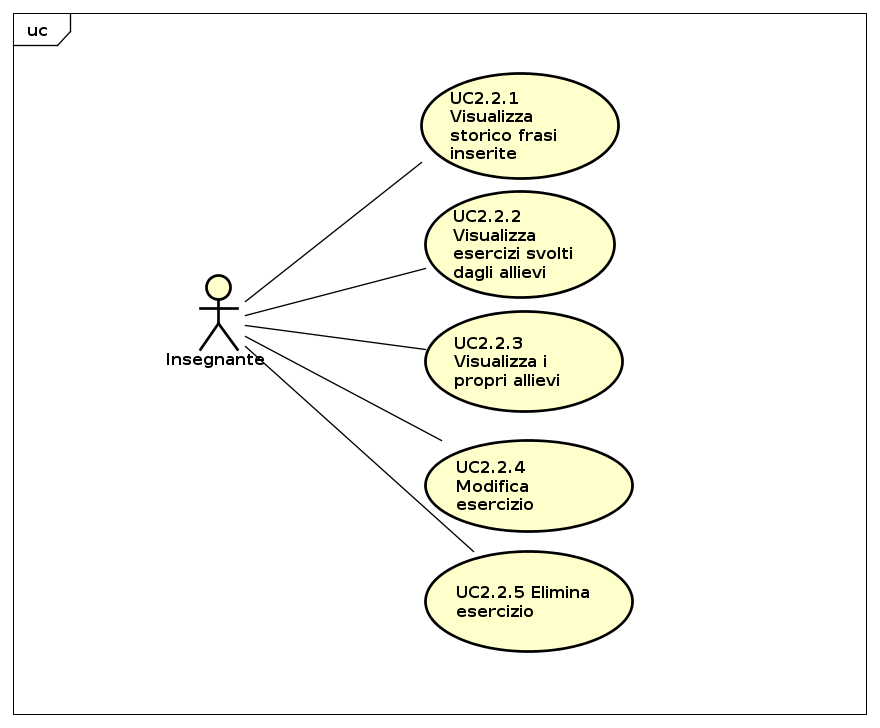
\includegraphics[width=17cm]{img/UC22.png} 
\caption{Caso d'uso UC2.2}
\end{figure}

\begin{itemize}
	\item[•] \textbf{Attori}: Insegnante;
	\item[•] \textbf{Descrizione}: L’insegnante visualizza il suo profilo personale;

	\item[•] \textbf{Precondizione}: Il sistema offre l’accesso a una dashboard con tutti i dati ;

	\item[•] \textbf{Postcondizione}:  Il profilo personale dell’insegnante è aperto;
	\item[•] \textbf{Flusso degli eventi}:
		\begin{enumerate}
			\item UC2.2.1 Visualizza storico frasi inserite;
			\item UC2.2.2 Visualizza esercizi svolti dagli allievi;
			\item UC2.2.3 Visualizza i propri allievi;
			\item UC2.2.4 Modifica esercizio;
			\item UC2.2.5 Elimina esercizio.
		\end{enumerate}
\end{itemize}

\subsection{UC2.2.1  Visualizza storico frasi inserite}

\begin{figure}[H]
\centering
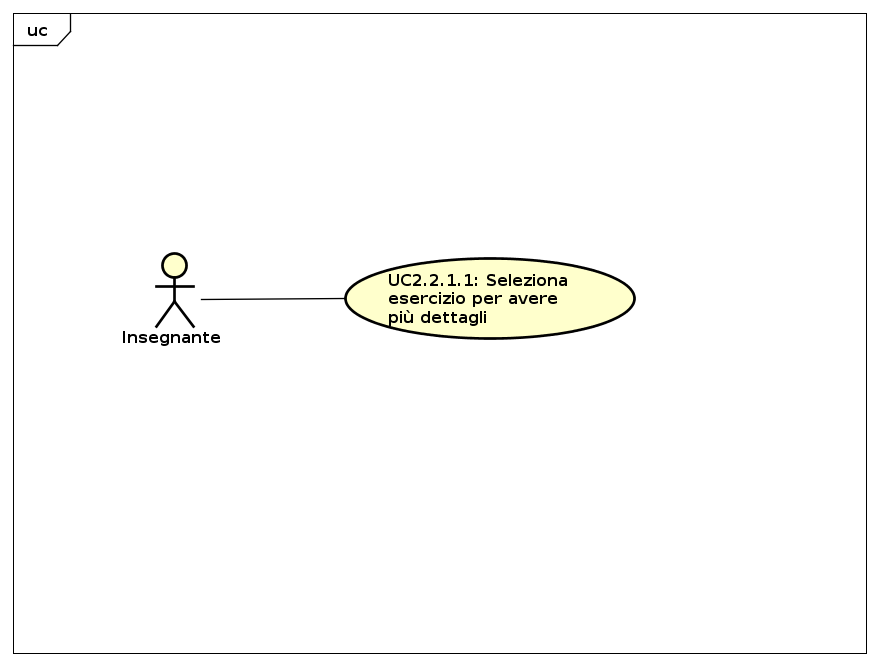
\includegraphics[width=10cm]{img/UC221.png} 
\caption{Caso d'uso UC2.2.1}
\end{figure}

\begin{itemize}
	\item[•] \textbf{Attori}:  Insegnante	\item[•] \textbf{Descrizione}: L’insegnante visualizza nel suo profilo personale lo storico delle frasi inserite; 
	\item[•] \textbf{Precondizione}: Il sistema offre la possibilità di visualizzare lo storico delle frasi inserite dall’insegnante;
	\item[•] \textbf{Postcondizione}:  L’insegnante può navigare all’interno della lista di frasi che ha inserito.
	\item[•] \textbf{Flusso degli eventi}:
		\begin{enumerate}
			\item UC2.2.1.1  Seleziona esercizio per avere più dettagli.
		\end{enumerate}
\end{itemize}

\subsection{UC2.2.1.1 Seleziona esercizio per avere più dettagli}
\begin{itemize}
	\item[•] \textbf{Attori}: Insegnante;
	\item[•] \textbf{Descrizione}:  L’insegnante seleziona dalla lista degli esercizi assegnati un esercizio e ne visualizza i dettagli;
	\item[•] \textbf{Precondizione}: Il sistema offre la possibilità di visualizzare i dettagli relativi ad un esercizio assegnato;
	\item[•] \textbf{Postcondizione}: L’insegnante legge le specifiche dell’esercizio selezionato.
\end{itemize}

\subsection{UC2.2.2  Visualizza esercizi svolti dagli allievi}
\begin{figure}[H]
\centering
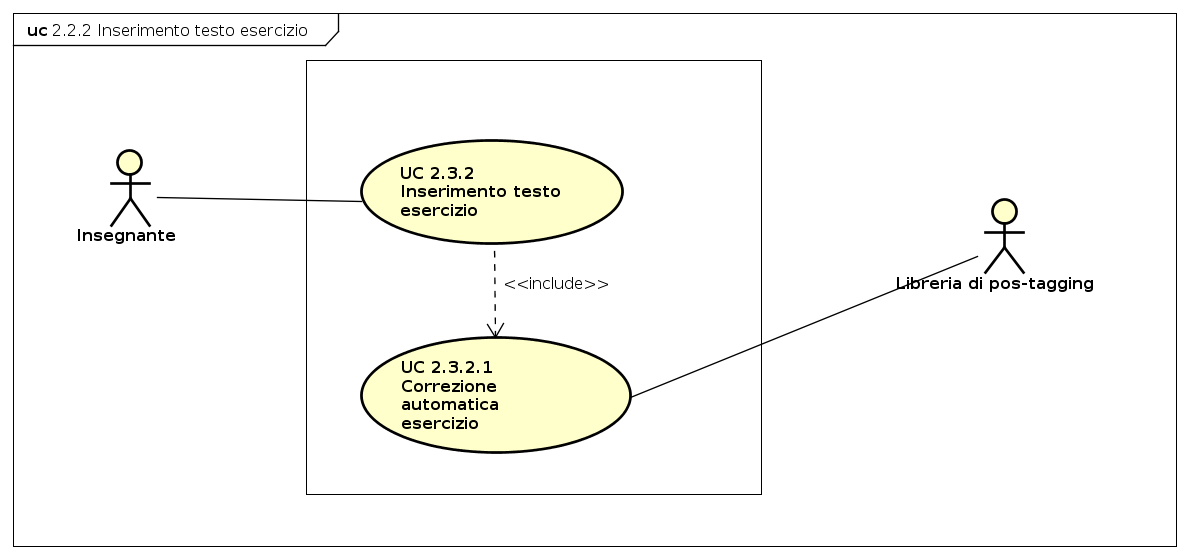
\includegraphics[width=10cm]{img/UC222.png} 
\caption{Caso d'uso UC2.2.2}
\end{figure}
\begin{itemize}
	\item[•] \textbf{Attori}:  Insegnante;
	\item[•] \textbf{Descrizione}:  L’insegnante è nella sezione profilo personale ed entra
		nel registro che conserva gli esercizi svolti dagli allievi;
	\item[•] \textbf{Precondizione}:  L’insegnante ha degli allievi e ha assegnato a loro degli esercizi che sono stati svolti e consegnati;

	\item[•] \textbf{Postcondizione}: L’insegnante può navigare all’interno degli esercizi svolti 
                       svolti dagli allievi; 

	\item[•] \textbf{Flusso degli eventi}:
		\begin{enumerate}
			\item UC2.2.1.1  Seleziona esercizio specifico per avere più dettagli.	
		\end{enumerate}
\end{itemize}

\subsection{UC2.2.3 Visualizza i propri allievi}

\begin{figure}[H]
\centering
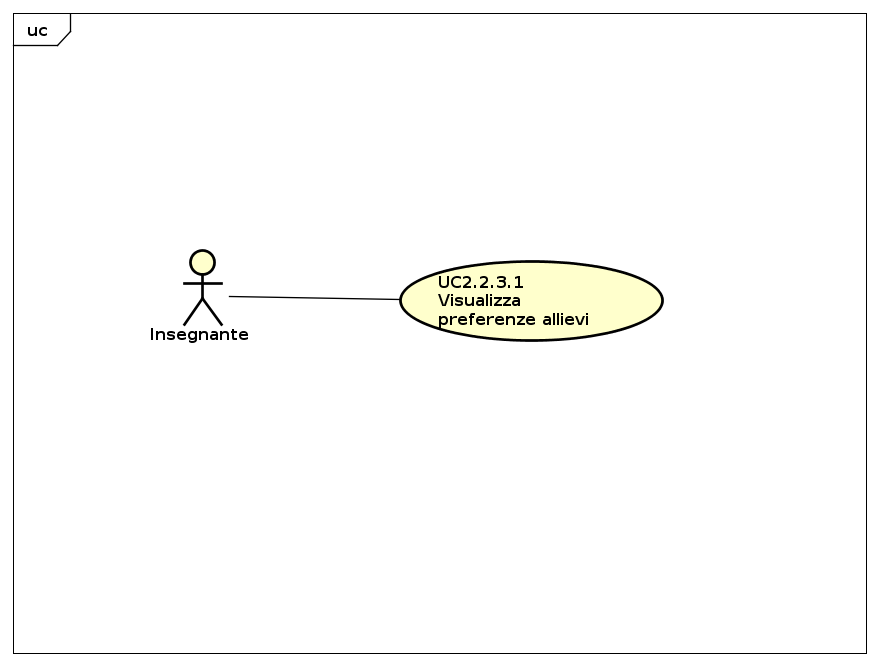
\includegraphics[width=10cm]{img/UC223.png} 
\caption{Caso d'uso UC2.2.3}
\end{figure}

\begin{itemize}
	\item[•] \textbf{Attori}: Insegnante;
	\item[•] \textbf{Descrizione}: L’insegnante visualizza la lista dei suoi allievi;
	\item[•] \textbf{Precondizione}: Il sistema offre all’insegnante di visualizzare la lista dei propri allievi;
	\item[•] \textbf{Postcondizione}: L’insegnante visualizza la lista dei propri allievi;
	\item[•] \textbf{Flusso degli eventi}:
		\begin{enumerate}
			\item UC2.2.3.1 Visualizza preferenze allievi.
		\end{enumerate}
\end{itemize}

\subsection{UC2.2.3.1 Visualizza preferenze allievi}
\begin{itemize}
	\item[•] \textbf{Attori}: Insegnante;
	\item[•] \textbf{Descrizione}: L’insegnante visualizza nel suo profilo personale le preferenze da parte degli allievi;
	\item[•] \textbf{Precondizione}: Il sistema offre la possibilità di poter segnare un insegnante come preferito;
	\item[•] \textbf{Postcondizione}: L’insegnante può vedere le preferenze degli allievi.
\end{itemize}


\subsection{UC2.2.4 Modifica esercizio}

\begin{figure}[H]
\centering
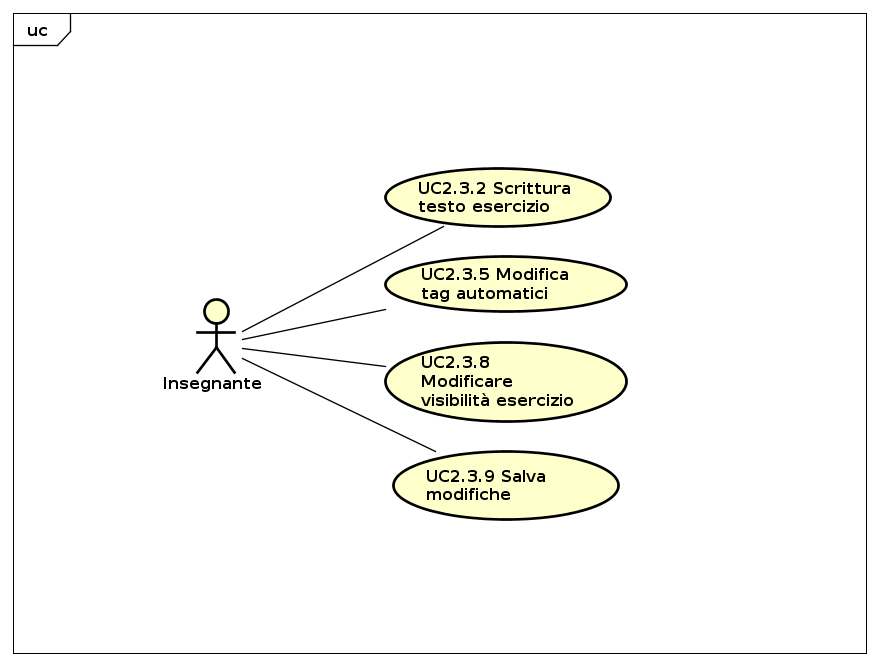
\includegraphics[width=10cm]{img/UC224.png} 
\caption{Caso d'uso UC2.2.4}
\end{figure}

\begin{itemize}
	\item[•] \textbf{Attori}: Insegnante;
	\item[•] \textbf{Descrizione}: L’insegnante può modificare un esercizio precedentemente inserito;
	\item[•] \textbf{Precondizione}: Il sistema offre la possibilità di modificare il testo, la
				lingua la visibilità i tag e le soluzioni alternative 
				dell’esercizio;
	\item[•] \textbf{Postcondizione}: L’esercizio è stato modificato;
	\item[•] \textbf{Flusso degli eventi}:
		\begin{enumerate}
			\item UC2.3.2 Scrittura testo esercizio;
			\item UC2.3.5 Modifica tag automatici;
			\item UC2.3.8 Modificare visibilità esercizio.
		\end{enumerate}
		    
\end{itemize}   	
	
\subsection{UC2.2.5 Elimina esercizio}
\begin{itemize}
	\item[•] \textbf{Attori}: Insegnante;
	\item[•] \textbf{Descrizione}: L’insegnante elimina un esercizio che è stato assegnato;
	\item[•] \textbf{Precondizione}: Il sistema offre la possibilità di eliminare un esercizio che è stato assegnato;
	\item[•] \textbf{Postcondizione}: L’esercizio assegnato è stato cancellato.
\end{itemize}


